\documentclass{article}

\usepackage{etoolbox}


\usepackage{fullpage}
\usepackage{color}
\usepackage{amsmath}
\usepackage{url}
\usepackage{verbatim}
\usepackage{graphicx}
\usepackage{parskip}
\usepackage{amssymb}
\usepackage{listings} % For displaying code
\lstset{
  tabsize=2,
  language=r,
  basicstyle=\ttfamily,
  % upquote=true,
  aboveskip={\baselineskip},
  columns=fixed,
  showstringspaces=false,
  extendedchars=true,
  breaklines=true,
  prebreak = \raisebox{0ex}[0ex][0ex]{\ensuremath{\hookleftarrow}},
  frame=false,
  showtabs=false,
  showspaces=false,
  showstringspaces=false,
  identifierstyle=\ttfamily,
  keywordstyle=\color[rgb]{0,0,1},
  commentstyle=\color[rgb]{0.07,0.472,0.07},
  stringstyle=\color[rgb]{0.627,0.126,0.941},
  language=matlab
  }

\begin{document}

\definecolor{blu}{rgb}{0,0,1}
\def\blu#1{{\color{blu}#1}}
\definecolor{gre}{rgb}{0,.5,0}
\def\gre#1{{\color{gre}#1}}
\definecolor{red}{rgb}{1,0,0}
\def\red#1{{\color{red}#1}}
\def\norm#1{\|#1\|}
\newcommand{\argmin}[1]{\mathop{\hbox{argmin}}_{#1}}
\newcommand{\argmax}[1]{\mathop{\hbox{argmax}}_{#1}}
\def\R{\mathbb{R}}
\newcommand{\fig}[2]{\includegraphics[width=#1\textwidth]{a3f/#2}}
\newcommand{\centerfig}[2]{\begin{center}\includegraphics[width=#1\textwidth]{a3f/#2}\end{center}}
\def\items#1{\begin{itemize}#1\end{itemize}}
\def\enum#1{\begin{enumerate}#1\end{enumerate}}
\def\argmax{\mathop{\rm arg\,max}}
\def\argmin{\mathop{\rm arg\,min}}
\def\half{\frac 1 2}
\newcommand{\code}[1]{\lstinputlisting[language=Matlab]{a3f/#1}}
\newcommand{\alignStar}[1]{\begin{align*}#1\end{align*}}
\newcommand{\mat}[1]{\begin{bmatrix}#1\end{bmatrix}}


%% Aaron's commands
\newcommand{\del}[2]{\ensuremath{\frac{\partial#1}{\partial#2}}}



\title{CPSC 540 Assignment 3 (due February 27)}
\author{Thibaut Astic}
\date{Student ID: 90142150; For Audit}
\maketitle



\section{Discrete and Gaussian Variables}

\subsection{MLE for General Discrete Distribution}

Consider a density estimation task, where we have two variables ($d=2$) that can each take one of $k$ discrete values. For example, we could have
\[
X = \mat{1 & 3\\4 & 2\\$k$ & 3\\1 & $k-1$}.
\]
The likelihood for example $x^i$ under a general discrete distribution would be
\[
p(x^i_1, x^i_2 | \Theta) = \theta_{x_1^i,x_2^i},
\]
where $\theta_{c_1,c_2}$ gives the probability of $x_1$ being in state $c_1$ and $x_2$ being in state $c_2$, for all the $k^2$ combinations of the two variables. In order for this to define a valid probability, we need all elements $\theta_{c_1,c_2}$ to be non-negative and they must sum to one, $\sum_{c_1=1}^k\sum_{c_2=1}^k \theta_{c_1,c_2} = 1$.
\enum{
\item Given $n$ training examples, \blu{derive the MLE for the $k^2$ elements of $\Theta$}.
\item Because of the sum-to-1 constraint, there are only $(k^2 - 1)$ degrees of freedom in the discrete distribution, and not $k^2$. \blu{Derive the MLE for this distribution assuming that
\[
\theta_{k,k} = 1 - \sum_{c_1=1}^k\sum_{c_2=1}^{k}\mathcal{I}[c_1\neq k,c_2 \neq k]\theta_{c_1,c_2},
\]
}so that the distribution only has $(k^2-1)$ parameters.
\item If we had separate parameter $\theta_{c_1}$ and $\theta_{c_2}$ for each variables, a reasonable choice of a prior would be a product of Dirichlet distributions,
\[
p(\theta_{c_1},\theta_{c_2}) \propto \theta_{c_1}^{\alpha_{c_1} - 1}\theta_{c_2}^{\alpha_{c_2} - 1}.
\]
For the general discrete distribution, a prior encoding the same assumptions  would be
\[
p(\theta_{c_1,c_2}) \propto \theta_{c_1,c_2}^{\alpha_{c_1} + \alpha_{c_2} - 2}.
\]
\blu{Derive the MAP estimate under this prior}.
}
Hint: it is convenient to write the likelihood for an example $i$ in the form
\[
p(x^i | \Theta) = \prod_{c \in [k]^2}\theta_c^{\mathcal{I}[x^i = c]},
\]
where $c$ is a vector containing $(c_1,c_2)$, $[x^i = c]$ evaluates to 1 if all elements are equal, and $[k]^2$ is all ordered pairs $(c_1,c_2)$. You can use the Lagrangian to enforce the sum-to-1 constraint on the log-likelihood, and you may find it convenient to define $N_c = \sum_{i=1}^n \mathcal{I}[x^i = c]$.


\textbf{Student's Solution:}

\begin{enumerate}
  %%%%%%%%%%%%%%%%%%%%%%%%%
  %% 1.1.1
  %%%%%%%%%%%%%%%%%%%%%%%%%
\item The MLE for a discrete distribution on $k^2$ elements
  $(j,\ell) \in [k]\times [k]$ is given by
  \begin{align*}
    \argmax_{0\leq \Theta \leq 1} p(X \mid \Theta) = \argmax_{\Theta\in [0,1]^k}
    \prod_{i=1}^n p(x^i_1, x^i_2 \mid \Theta) = \argmax_{\Theta \in [0,1]^k}
    \prod_{j,\ell \in [k]} \theta_{j,\ell}^{N_{j,\ell}}
  \end{align*}
  where $N_{j,\ell} := \#\{ i \in [n] : x^i_1 = j \And x^i_2 = \ell \}$ and
  $0 \leq \Theta \leq 1$ is multi-index notation for
  $\Theta \in [0,1]^k$.

  %%%%%%%%%%%%%%%%%%%%%%%%%
  %% 1.1.2
  %%%%%%%%%%%%%%%%%%%%%%%%%
\item From above we see that the assumption for this question yields, where $J
  := \{ (j,\ell) \in [k]^2 : j, \ell \neq k\}$,
  \begin{align*}
    \argmax_{0 \leq \Theta \leq 1} p(X \mid \Theta) = \argmax_{0 \leq \Theta
    \leq 1} \big( 1 - \sum_{j, \ell \in J} \theta_{j, \ell} \big)^{N_{k,k}} \prod_{j,\ell \in J} \theta_{j, \ell}^{N_{j,\ell}}
  \end{align*}
  Then the MLE can be determined by finding the critical point of the
  log-likelihood (since $\log$ is a concave function, hence does not change the
  maximizer). For $\lambda \in J$,
  \begin{align*}
    0 &= \del{}{\theta_\lambda} \log \mathcal{L}(\Theta \mid X) =
        N_{k,k}\del{}{\theta_\lambda} \log\big(1 -
        \sum_{j,\ell \in J} \theta_{j,\ell}\big)
        + \del{}{\theta_\lambda} \sum_{j,\ell \in J} N_{j, \ell} \log \theta_{j, \ell}
    \\
      &= \frac{-N_{k,k}}{1 - \sum_{j,\ell \in J}\theta_{j,\ell}} +
        \frac{N_\lambda}{\theta_\lambda}
  \end{align*}
  Hence, letting
  $J(j,\ell) := \{(m,n) \in [k]\times [k] : (m,n) \neq (k,k), (m,n) \neq
  (j,\ell)\}$,
  \begin{align*}
    \frac{N_\lambda}{\theta_\lambda} = \frac{N_{k,k}}{1 - \sum_{j,\ell \in J}
    \theta_{j,\ell}} \quad \implies \quad \frac{\theta_\lambda}{1 -\sum_{j,\ell
    \in J} \theta_{j,\ell}} = \frac{N_\lambda}{N_{k,k}}
  \end{align*}
  thereby implying, since selecting $(k,k)$ above was arbitrary,
  \begin{align*}
    \theta_\lambda := \frac{N_\lambda}{\sum_{j,\ell \in [k]^2} N_{j,\ell}}
  \end{align*}

  %%%%%%%%%%%%%%%%%%%%%%%%% 
  %% 1.1.3
  %%%%%%%%%%%%%%%%%%%%%%%%%
\item Let assume a prior such that:
 \[
 p(\theta_{c_1,c_2}) \propto \theta_{c_1,c_2}^{\alpha_{c_1} + \alpha_{c_2} - 2}.
 \]
 Then the MAP estimate can be written using Bayes rule :
 \[
 \argmax_{0 \leq \Theta \leq 1} p(\Theta|X) \propto  \argmax_{0 \leq \Theta \leq 1} p(X|\Theta) p(\Theta)
 \]
 We can then determine it by finding the critical point of the negative log-likehood and use a Lagrangian with multiplier $\Lambda$ to apply the constrain from question 2. We then have
 \[
 - \nabla_{\theta_{c}} \mathcal{L}(\Theta)  = \nabla_{\theta_{c}} \left(-\sum_{i=1}^n \log(\theta_{x_1^i,x_2^i}) - \sum_{c_1=1}^k\sum_{c_2=1}^k \theta_{c_1,c_2} log(\theta_{c_1,c_2}^{\alpha_{c_1} + \alpha_{c_2}- 2}) + \Lambda (\sum_{c_1=1}^k\sum_{c_2=1}^k \theta_{c_1,c_2} \theta_{c_1,c_2}^{\alpha_{c_1} + \alpha_{c_2} - 2} -1)\right) = 0
 \]

 \[
 \sum_{i=1}^n \mathcal{I}[x^i_1 = c_1,x^i_2 = c_2] \frac{1}{\theta_{c_1,c_2}}+(\alpha_{c_1} + \alpha_{c_2}- 2)+\frac{1}{\theta_{c_1,c_2}} - \Lambda = 0
 \]
 which gives us:
 \[
 \theta_{c_1,c_2} = \frac{N_c+\alpha_{c_1} +\alpha_{c_2}- 2}{\Lambda}
 \]
 And the constrain on the sum up allow us to solve for $\Lambda$ and we finally get:
  \[ 
  \theta_{c_1,c_2} = \frac{N_c+\alpha_{c_1} +\alpha_{c_2}- 2}{\sum_{j,\ell \in [k]^2} (N_{j,\ell}+\alpha_j+\alpha_{\ell}-2)}
 \]

\end{enumerate}

\subsection{Generative Classifiers with Gaussian Assumption}

Consider the 3-class classification dataset in this image:
\centerfig{.4}{sample.png}
In this dataset, we have 2 features and each colour represents one of the classes. Note that the classes are highly-structured: the colours each roughly follow a Gausian distribution plus some noisy samples.

Since we have an idea of what the features look like for each class, we might consider classifying  inputs $x$ using a \emph{generative classifier}. In particular, we are going to use Bayes rule to write
\[
p(y=c|x,\Theta) = \frac{p(x| y=c, \Theta) \cdot p(y=c|\Theta)}{p(x|\Theta)},
\]
where $\Theta$ represents the parameters of our model. To classify a new example $\hat{x}$, generative classifiers would use
\[
\hat{y} = \argmax_{y \in \{1,2,\dots,k\}} p(\hat{x}| y=c,\Theta)p(y=c|\Theta),
\]
where in our case the total number of classes $k$ is $3$ (The denominator $p(\hat{x}|\Theta)$ is irrelevant to the classification since it is the same for all $y$.)
% and $\theta_c$ is the set of parameters associated class $c$.
Modeling $p(y=c|\Theta)$ is eays: we can just use a $k$-state categorical distribution,
\[
p(y = c | \Theta) = \theta_c,
\]
where $\theta_c$ is a single parameter for class $c$. The maximum likelihood estimate of $\theta_c$ is given by $n_c/n$, the number of times we have $y^i = c$ (which we've called $n_c$) divided by the total number of data points $n$.

Modeling $p(x | y =c, \Theta)$ is the hard part: we need to know the \emph{probability of seeing the feature vector $x$ given that we are in class $c$}. This corresponds to solving a density estimation problem for each of the $k$ possible classes. 
To make the density estimation problem tractable, we'll assume that the distribution of $x$ given that $y=c$ is given by a $\mathcal{N}(\mu_c,\Sigma_c)$ Gaussian distribution for a class-specific $\mu_c$ and $\Sigma_c$,
\[
p(x | y=c, \Theta) = \frac{1}{(2\pi)^{\frac{d}{2}}|\Sigma_c|^{\half}}\exp\left(-\half (x-\mu_c)^T\Sigma_c^{-1}(x-\mu_c)\right).
\]
Since we are distinguishing between the probability under $k$ different Gaussians to make our classification, this is called \emph{Gaussian discriminant analysis} (GDA). In the special case where we have a constant $\Sigma_c = \Sigma$ across all classes it is known as \emph{linear discriminant analysis} (LDA) since it leads to a linear classifier between any two classes (while the region of space assigned to each class forms a convex polyhedron as in $k$-means clustering). Another common restriction on the $\Sigma_c$ is that they are diagonal matrices, since this only requires $O(d)$ parameters instead of $O(d^2)$ (corresponding to assuming that the features are independent univariate Gaussians given the class label).
Given a dataset $\mathcal{D}=\{(x^i, y^i)\}_{i=1}^n$, where $x^i\in\R^d$ and $y^i\in\{1,\ldots,k\}$, the maximum likelihood estimate (MLE) for the $\mu_c$ and $\Sigma_c$ in the GDA model is the solution to
\[
\argmax_{\mu_1,\mu_2,\dots,\mu_k,\Sigma_1,\Sigma_2,\dots,\Sigma_k} \prod_{i=1}^n p(x^i | y^i, \mu_{y^i},\Sigma_{y^i}).
\]
This means that the negative log-likelihood will be  equal to
\alignStar{
- \log p(X|y,\Theta) & = -\sum_{i=1}^n \log p(x^i | y^i | \mu_{y^i},\Sigma_{y^i})\\
& = \sum_{i=1}^n \frac{1}{2}(x^i - \mu_{y^i})^T\Sigma_{y^i}^{-1}(x^i - \mu_{y^i}) + \half\sum_{i=1}^n \log|\Sigma_{y^i}| + \text{const.}
}

\enum{
\item \blu{Derive the MLE for the GDA model under the assumption of \emph{common diagonal covariance} matrices}, $\Sigma_c = D$ ($d$ parameters). (Each class will have its own mean $\mu_c$.)
\item \blu{Derive the MLE for the GDA model under the assumption of \emph{individual scale-identity} matrices}, $\Sigma_c = \sigma_c^2 I$ ($k$ parameters).
\item It's painful to derive these from scratch, but you should be able to see a pattern that would allow other common restrictions. Without deriving the result from scratch (hopefully), \blu{give the MLE for the case of \emph{individual full} covariance matrices}, $\Sigma_c$ ($O(kd^2)$ parameters).
\item When you run \emph{example\_generative} it loads a variant of the dataset in the figure that has 12 features and 10 classes. This data has been split up into a training and test set, and the code fits a $k$-nearest neighbour classifier to the training set then reports the accuracy on the test data ($\sim 36\%$). The $k$-nearest neighbour model does poorly here since it doesn't take into account the Gaussian-like structure in feature space for each class label. Write a function \emph{generativeGaussian} that fits a GDA model to this dataset (using individual full covariance matrices). \blu{Hand in the function and report the test set accuracy}.
\item In this question we would like to replace the Gaussian distribution of the previous problem with the more robust multivariate-t distribution so that it isn't influenced as much by the noisy data.
Unlike the previous case, we don't have a closed-form solution for the parameters. However, if you run \emph{example\_tdist} it generates random noisy data and fits a multivariate-t model (you will need to add the \emph{minFunc} directory to the Matlab path for the demo to work). By using the \emph{multivariateT} model, write a new function \emph{generativeStudent} that implements a generative model that is based on the multivariate-t distribution instead of the Gaussian distribution. \blu{Report the test accuracy  with this model.}
}
Hints: you will be able to substantially simplify the notation in parts 1-3 if you use the notation $\sum_{i \in y_c}$ to mean the sum over all values $i$ where $y^i = c$. Similarly, you can use $n_c$ to denote the number of cases where $y_i = c$, so that we have $\sum_{i \in y_c}1 = n_c$. Note that the determinant of a diagonal matrix is the product of the diagonal entries, and the inverse of a diagonal matrix is a diagonal matrix with the reciprocals of the original matrix along the diagonal. For part three you can use the result from class regarding the MLE of a general multivariate Gaussian. You may find it helpful to use the included \emph{logdet.m} function to compute the log-determinant in more numerically-stable way.


\textbf{Student's Solution:}
\begin{enumerate}
  %%%%%%%%%%%%%%%%%%%%%%%%%
  %% 1.2.1
  %%%%%%%%%%%%%%%%%%%%%%%%%
\item Derive the MLE for the GDA model under the assumption of common diagonal covariance matrices $\Sigma_c = D$ ($d$ parameters). (Each class will have its own mean $\mu_c$.)
  
 We first start to get the MLE in respect with $\mu_c$. We take the gradient of the negative log-likelihood with respect to $\mu_c$ an set it to zero:
 \alignStar{
 - \nabla_{\mu_c} \log p(X|y,\Theta) & = - \nabla_{\mu_c} \sum_{i=1}^n \log p(x^i | y^i | \mu_{y^i},\Sigma_{y^i})\\
 & = \sum_{i=1}^n \mathcal{I}[y^i=c] \Sigma_{y^i}^{-1}(x^i - \mu_{y^i})
 }
 \[ - \nabla_{\mu_c} \log p(X|y,\Theta)  = 0 \implies \mu_c= \frac{1}{n_c}\sum_{i=1}^n \mathcal{I}[y^i=c] x^i \]

 We then can use this result for $\mu_c$ to get the MLE for the covariances matrices under the assumption of common diagonal covariance matrices. Using the derivation seen in class, we reparametrize the MLE in term of the precision matrix $\Phi = \Sigma^{-1}$ and the all samples covariance matrix $S = \frac{1}{n} \sum_{i=1}^n (x^i - \mu_{y^i})(x^i - \mu_{y^i})^T$:
 \[- \log p(X|y,\Theta)  = \frac{n}{2} Tr(S \Phi) - \frac{n}{2} log|\Phi| \]
 We now put in our assumption of common diagonal covariance matrices, we only to derive the diagonal elements, the others are by assumption equal to 0, which implies:
 \alignStar{- \nabla_{D^{-1} = \Phi} \log p(X|y,\Theta) & = \nabla_{D^{-1} = \Phi}(\frac{n}{2} Tr(S \Phi) - \frac{n}{2} log|\Phi|) \\
 & =  \frac{n}{2} diag(S) - \frac{n}{2} D
 }
 Which gives us the following result:
 \[
 \frac{n}{2} diag(S) - \frac{n}{2} = 0 \implies \\
 D = diag(S)
 \]
  %%%%%%%%%%%%%%%%%%%%%%%%%
  %% 1.2.2
  %%%%%%%%%%%%%%%%%%%%%%%%%
\item Derive the MLE for the GDA model under the assumption of \emph{individual scale-identity matrices}, $\Sigma_c = \sigma_c^2 I$ ($k$ parameters)
 
 We will first notice that changing assumption on $\Sigma_c$ does not change the MLE for $\mu_c$.
 We then notice that here our assumption on the covariance matrix is strong, in the sense that we impose all the diagonal terms to be equal. We cannot use the reparametrization used earlier.
 \alignStar{
 - \log p(X|y,\Theta) & = \sum_{i=1}^n \frac{1}{2}\sigma_{y^i}^{-2}(x^i - \mu_{y^i})^T(x^i - \mu_{y^i}) + \half\sum_{i=1}^n \log|\sigma^2_{y^i}| + \text{const.} \\
 - \nabla_{\sigma_c^2} \log p(X|y,\Theta) & = \frac{1}{2 \sigma_c^4} \sum_{i=1}^n \mathcal{I}[y^i=c] (x^i - \mu_{y^i})^T(x^i - \mu_{y^i}) + \frac{n_c}{2} \sigma_c^{-2} \\
 }
 which gives us the result:
  \[
 - \nabla_{\sigma_c^2} \log p(X|y,\Theta) = 0 \implies \\
 \sigma_c^2 = \frac{1}{n_c} \sum_{i=1}^n \mathcal{I}[y^i=c] (x^i - \mu_{y^i})^T(x^i - \mu_{y^i})
 \]
  %%%%%%%%%%%%%%%%%%%%%%%%%
  %% 1.2.3
  %%%%%%%%%%%%%%%%%%%%%%%%%
 \item Without derivation, give the MLE for the case of \emph{individual full} covariance matrices
 Your intuition in that case is:
 \[
 \Sigma_c = \frac{1}{n_c} \sum_{i=1}^n \mathcal{I}[y^i=c] (x^i - \mu_{y^i})(x^i - \mu_{y^i})^T
 \]
  %%%%%%%%%%%%%%%%%%%%%%%%%
  %% 1.2.4
  %%%%%%%%%%%%%%%%%%%%%%%%%
 \item  Write a function \emph{generativeGaussian} that fits a GDA model to this dataset (using individual full covariance matrices). \blu{Hand in the function and report the test set accuracy}.

 \lstinputlisting{./a3/generativeGaussian.m}

 Our test set accuracy is now 0.63.
  %%%%%%%%%%%%%%%%%%%%%%%%%
  %% 1.2.5
  %%%%%%%%%%%%%%%%%%%%%%%%%
 \item Write a new function \emph{generativeStudent} that implements a generative model that is based on the multivariate-t distribution instead of the Gaussian distribution. \blu{Report the test accuracy  with this model.} 
 \lstinputlisting{./a3/generativeStudent.m}

 Our test set accuracy is now 0.79.

 \begin{tabular}[h]{cccc}
  \textbf{Method} & \textbf{Accuracy}\\
  KNN & 0.37\\
  GDA & 0.63\\
  Student & 0.79
\end{tabular}

\end{enumerate}

\subsection{Self-Conjugacy for the Mean Parameter}

If $x$ is distributed according to a Gaussian with mean $\mu$,
\[
x \sim \mathcal{N}(\mu,\sigma^2),
\]
and we assume that $\mu$ itself is distributed according to a Gaussian
\[
\mu \sim \mathcal{N}(\alpha,\gamma^2),
\]
then the posterior $\mu | x$ also follows a Gaussian distribution.\footnote{We say that the Gaussian distribution is the `conjugate prior' for the Gaussian mean parameter (we'll formally discuss conjugate priors later in the course). Another reason the Gaussian distribution is important is that is the only (non-trivial) continuous distribution that has this `self-conjugacy' property.} \blu{Derive the form of the (Gaussian) distribution for $p(\mu|x,\alpha,\sigma^2,\gamma^2)$.} %You can assume that $\sigma=1$ and $\gamma=1$.

Hints: Use Bayes rule and use the $\propto$ sign to get rid of factors that don't depend on $\mu$. You can ``complete the square'' to make the product look like a Gaussian distribution, e.g. when you have $\exp(ax^2 - bx + \text{const})$ you can factor out an $a$ and add/subtract $(b/2a)^2$ to re-write it as
\begin{align*}
\exp\left(ax^2 - bx + const\right) & \propto
\exp\left(ax^2 - bx\right) = \exp\left(a(x^2 - (b/a)x)\right) \\& \propto \exp\left(a(x^2 - (b/a)x + (b/2a)^2)\right) =  \exp\left(a(x - (b/2a))^2\right).
\end{align*}
Note that multiplying by factors that do not depend on $\mu$ within the exponent does not change the distribution. In this question you will want to complete the square to get the distribution on $\mu$, rather than $x$.
You may find it easier to solve thie problem if you parameterize the Gaussians in terms of their `precision' parameters (e.g., $\lambda = 1/\sigma^2$, $\lambda_0 = 1/\gamma^2$) rather than their variances $\sigma^2$ and $\gamma^2$.

\newpage

\textbf{Student's Solution:}

Re-using Tutorial 6 material, we get:
\begin{align}
p(\mu | x,\alpha, \sigma^2, \gamma^2) &= p(x| \mu, \alpha, \sigma^2, \gamma^2)p(\mu| \alpha,  \gamma^2) / Z \qquad\text{(Bayes rule)}\\
&= p(x| \mu, \sigma^2)p(\mu| \alpha,  \gamma^2) / Z \qquad\text{(Conditional independence)}\\
&\propto p(x| \mu, \sigma^2)p(\mu| \alpha,  \gamma^2) \qquad\text{(Dropping the }Z)\\
&\propto \exp\left(-\frac{(x - \mu)^2}{2\sigma^2}\right)\exp\left(-\frac{(\mu - \alpha)^2}{2\gamma^2}\right) \qquad\text{(Subbing in the expression for the pdf and dropping constants)}\\
&= \exp\left(-\frac{(x - \mu)^2}{2\sigma^2}-\frac{(\mu - \alpha)^2}{2\gamma^2}\right) \\
&= \exp\left(-\left( \frac{\sigma^2+\gamma^2}{2(\sigma\gamma)^2} \mu^2 - 2\frac{\gamma^2x+\sigma^2\alpha}{(\sigma\gamma)^2}\mu\right)\right) \qquad\text{(developing the expression and dropping constants)}\\
&= \exp\left(- \frac{\sigma^2+\gamma^2}{2(\sigma\gamma)^2} \left(\mu-\frac{\gamma^2x+\sigma^2\alpha}{\sigma^2+\gamma^2}\right)^2\right) \qquad\text{(Factorization and final result)}
\end{align}

So the posterior follows a Gaussian distribution 
\[
p(\mu|x,\alpha,\sigma^2,\gamma^2) \sim \mathcal{N}(\frac{\gamma^2x+\sigma^2\alpha}{\sigma^2+\gamma^2},\frac{(\sigma\gamma)^2}{\sigma^2+\gamma^2}),
\]



\section{Mixture Models and Expectation Maximization}

\subsection{Semi-Supervised Gaussian Discriminant Analysis}

Consider fitting a GDA model where some of the $y^i$ values are missing at random. In particular, let's assume we have $n$ labeled examples $(x^i,y^i)$ and then another another $t$ unlabeled examples $(x^i)$. This is a special case of \emph{semi-supervised learning}, and fitting generative models with EM is one of the oldest semi-supervised learning techqniues. When the classes exhibit clear structure in the feature space, it can be very effective even if the number of labeled examples is very small.

\enum{
\item \blu{Derive the EM update for fitting the parameters of a GDA model (with individual full covariance matrices) in the semi-superivsed setting where we have $n$ labeled examples and $t$ unlabeled examples}.
\item If you run the demo \emph{example\_SSL}, it will load a variant of the dataset from the previous question, but where the number of labeled examples is small and a large number of unlabeled examples are available. The demo first fits a KNN model and then a generative Gaussian model (once you are finished Question 1).
Because the number of labeled examples it quite small, the performance is worse than in Question 2. Write a function \emph{generativeGaussianSSL} that fits the generative Gaussian model of the previous question using EM to incorporate the unlabeled data. \blu{Hand in the function and report the test error when training on the full dataset}.
\item Repeat the previous part, but using the ``hard''-EM algorithm where we explicitly classify all the unlabeled examples. \blu{How does this change the performance and the number of iterations}?
}

Hint: for the first question most of the work has been done for you in the EM notes on the course webpage. You can use the result (**) and the update of $\theta_c$ from those notes, but you will need to work out the update of the parameters of the Gaussian distribution $p(x^i | y^i, \Theta)$.

Hint: for the second question, although EM often leads to simple updates, implementing them correctly can often be a pain. One way to help debug your code is to compute the observed-data log-likelihood after every iteration. If this number goes down, then you know your implementation has a problem. You can also test your updates of sets of variables in this way too. For example, if you hold the $\mu_c$ and $\Sigma_c$ fixed and only update the $\theta_c$, then the log-liklihood should not go down. In this way, you can test each of combinationso of updates on their to make sure they are correct.

\textbf{Student's Solution:}
\begin{enumerate}
  %%%%%%%%%%%%%%%%%%%%%%%%%
  %% 2.1.1
  %%%%%%%%%%%%%%%%%%%%%%%%%
  \item Starting from equation (**) from the note:
  \[
  Q(\theta|\theta_k) =  \sum_{i=1}^n \log p(y_i ,x_i |\theta)+ \sum_{i=1}^t\sum_{\tilde{y}_i\in\{0,1\}} r_{\tilde{y}_i}^i\log p(\tilde{y}_i ,\tilde{x}_i |\theta).
  \]
  we now want to update for $\mu_c,\Sigma_c$ and $\theta_c$, with $c$ the class index.
  The update for $\mu_i$ has been developed in the tutorial and we are reproducing it here.
  \begin{align}
  \nabla_{\mu_c} Q(\theta|\theta_k) &=  \sum_{i=1}^n \mathbb{I}(y_i = c)\Sigma_c^{-1}(x_i - \mu_c) + \sum_{i=1}^t\sum_{\tilde{y}_i\in\{0,c\}} r_{\tilde{y}_i}^i \mathbb{I}(y_i = c)\Sigma_c^{-1}(x_i - \mu_c).\\
  &=  \sum_{i=1}^n \mathbb{I}(y_i = c)\Sigma_c^{-1}(x_i - \mu_c) + \sum_{i=1}^t r_{c}^i\Sigma_c^{-1}(x_i - \mu_c).\\
  \end{align}
  Setting it to 0, we get
  \begin{align}
 \sum_{i=1}^n \mathbb{I}(y_i = c)\Sigma_c^{-1}(x_i - \mu_c) &+ \sum_{i=1}^t r_{c}^i\Sigma_c^{-1}(x_i - \mu_c) = 0\\
  \sum_{i=1}^n \mathbb{I}(y_i = c)x_i + \sum_{i=1}^t r_{c}^i x_i & =  \mu_c \sum_{i=1}^n \mathbb{I}(y_i = c)  +   \sum_{i=1}^t r_{c}^i\mu_c \\
  \mu_c &= \frac{1}{n_c + r_{c}} ( \sum_{i=1}^n \mathbb{I}(y_i = c)x_i + \sum_{i=1}^t r_{c}^i x_i ) \\
  \end{align}
  With $r_{c} = \sum_{i=1}^t r_{c}^i$.

  We derive $Sigma_c$ the same way, under full matrices assumptions:
  \begin{align}
  \nabla_{\Sigma_c} Q(\theta|\theta_k) &=  \frac{1}{2}\sum_{i=1}^n \mathbb{I}(y_i = c)(x_i - \mu_c)(x_i - \mu_c)^T -\frac{1}{2}\sum_{i=1}^n \mathbb{I}(y_i = c)\Sigma_c \\
  & + \frac{1}{2}\sum_{i=1}^t\sum_{\tilde{y}_i\in\{0,c\}} r_{\tilde{y}_i}^i \mathbb{I}(y_i = c)(x_i - \mu_c)(x_i - \mu_c)^T-\frac{1}{2}\sum_{i=1}^t\sum_{\tilde{y}_i\in\{0,c\}} r_{\tilde{y}_i}^i \mathbb{I}(y_i = c)\Sigma_c.\\
  \Sigma_c &=  \frac{1}{N_c+r_c}\left(\sum_{i=1}^n \mathbb{I}(y_i = c)(x_i - \mu_c)(x_i - \mu_c)^T + \sum_{i=1}^t r_{c}^i (x_i - \mu_c)(x_i - \mu_c)^T \right).\\
  \end{align}

  and Finally for $\theta_c$ the result was already derived in the EM notes:
  \[
 \theta_c = \frac{N_c+r_c}{n+t}
  \]

  %%%%%%%%%%%%%%%%%%%%%%%%%
  %% 2.1.1
  %%%%%%%%%%%%%%%%%%%%%%%%%
 \item
 Our function generativeGaussianSSL that perform E and M steps of EM to fit a mixture of gaussian. The predic 
  \lstinputlisting{./a3/generativeGaussianSSL.m}
  
  \begin{tabular}[h]{cccc}
  \textbf{Method} & \textbf{Accuracy}\\
  KNN & 0.28\\
  GDA & 0.54\\
  SSL Gaussian Soft-EM & 0.75 \\
  SSL Gaussian Hard-EM & 0.76 
\end{tabular}
 
 The improvement with EM is significant. We almost have the same accuracy than in the case of fully labeled data.
  %%%%%%%%%%%%%%%%%%%%%%%%%
  %% 2.1.1
  %%%%%%%%%%%%%%%%%%%%%%%%%
 \item
  The accuracy is slightly better with Hard-EM but not much. Our hypothesis is that soft-EM can blur the results if the classes are not very distinctive. the number of iteration to reach a plateau in accuracy is slgihtly the same here. 
  
  \centerfig{.7}{SoftHard_Iterations_EM.jpg}

\end{enumerate}

\subsection{Mixture of Bernoullis}

The function \emph{example\_Bernoulli} loads a binarized version of the MNIST dataset and fits a density model that uses an independent Bernoulli to model each feature. If the reports the average NLL on the test data and shows 4 samples generated from the model. Unfortunately, the test NLL is infinity and the samples look terrible.
\enum{
\item To address the problem that the average NLL is infinity, modify the \emph{densityBernoulli} function to implement Laplace smoothing based on an extra argument $\alpha$. \blu{Hand in the code and report the average NLL with $\alpha = 1$}.
\item Write a new function implementing the mixture of Bernoullis model with Laplace smoothing of the $\theta$ values (note that Laplace smoothing only change the M-step). \blu{Hand in the code and report the average NLL with $\alpha = 1$ and $k=10$ for a particular run of the algorithm, as well as 4 samples from the model and 4 of the cluster images.}
}

\textbf{Student's Solution:}
\begin{enumerate}
  %%%%%%%%%%%%%%%%%%%%%%%%%
  %% 2.2.1
  %%%%%%%%%%%%%%%%%%%%%%%%%
  \item Our code with Laplace Smoothing (we used the generalization showned in class with both $\alpha$ and $\beta$). NLL is about 205 now. The samples have not really change.

  \lstinputlisting{./a3/densityBernoulli.m}

  %%%%%%%%%%%%%%%%%%%%%%%%%
  %% 2.2.2
  %%%%%%%%%%%%%%%%%%%%%%%%%
  \item We admit we did not quite succeed to implement these methods. The difficulty came mainly from underflowing in the formulation of log(r), despite using successfully the log-sum-exp trcik. The effect is to assign all the samples to the same cluster after just a few iterations, reproducing a simple independent Bernoulli. The results we are showing here are from a pick before such a numerical issue after just a couple iterations. But already we see that the cluster looks like numbers and we have more spatial coherence in the samples. We tested our code on more trivial datasets and was successful in recovering the parameters. We will be very eager to have some feedback on it and see what was the way to deal with this r parameters to avoid the algorithm to put everything in the same cluster. Thanks!

    \lstinputlisting{./a3/mixtureBernoulli.m}

\begin{figure}[!ht]
%\vspace{-10pt}
\centering
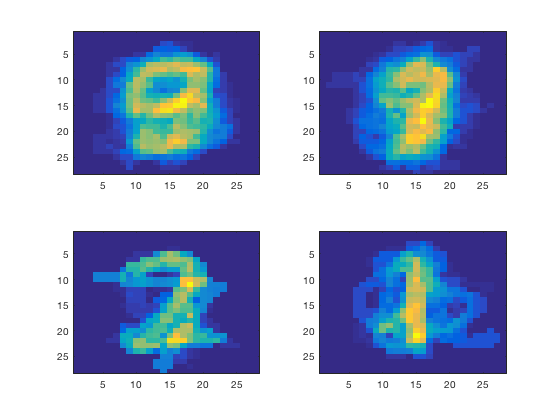
\includegraphics[scale=0.5]{./a3/cluster.png}
\caption{Cluster Images}
\label{cluster}
%\vspace{-40pt}
\end{figure}

\begin{figure}[!ht]
%\vspace{-10pt}
\centering
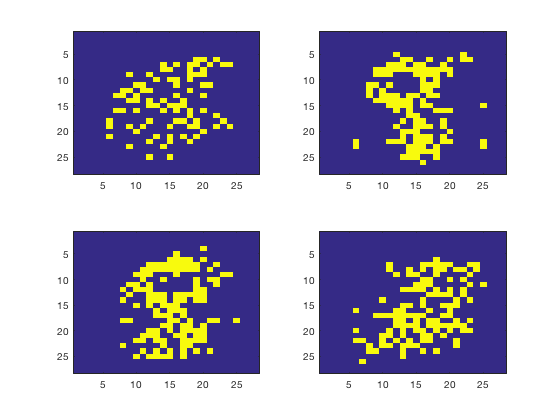
\includegraphics[scale=0.5]{./a3/Samples.png}
\caption{Samples}
\label{Samples}
%\vspace{-40pt}
\end{figure}

\end{enumerate}

\newpage
\newpage

\subsection{Project Proposal}

As an auditor, I do not want to submit one.

\end{document}
%%% Local Variables:
%%% mode: latex
%%% TeX-master: t
%%% End:
